\chapter{Constraint Satisfaction}
In this chapter we discuss algorithms for solving \emph{\color{blue}constraint satisfaction problems}.
This chapter is structured as follows:
\begin{enumerate}
\item The first section defines the notion of a constraint satisfaction problem.  In order to illustrate this
      concept, two examples of constraint satisfaction problems are presented.  After that, we discuss
      applications of constraint satisfaction problems.
\item The simplest algorithm to solve a constraint satisfaction problem is via \emph{\color{blue}brute force search}.
      The idea behind brute force search is to test all possible variable assignments.
\item In most cases, the search space is too big to be enumerated completely.
      \emph{\color{blue}Backtracking search} improves on brute force search by mixing the generation
      of assignments with the testing of the constraints.  In most cases, this approach can
      drastically improve the performance of the search algorithm.
\item Backtracking search can be refined by using \emph{\color{blue}constraint propagation} and by
      using the \emph{\color{blue}most restricted variable} heuristic.
\item Furthermore, checking the \emph{\color{blue}consistency} of the values assigned to different variables
      can reduce the size of the search space considerably. 
\item Finally, \emph{\color{blue}local search} is a completely different approach to solve
      constraint satisfaction problems.
\end{enumerate}

\section{Formal Definition of Constraint Satisfaction Problems}
Formally, we define a 
\href{https://en.wikipedia.org/wiki/Constraint_satisfaction_problem}{constraint satisfaction problem} as a triple
\\[0.2cm]
\hspace*{1.3cm}
$\mathcal{P} := \langle \mathtt{Vars}, \mathtt{Values}, \mathtt{Constraints} \rangle$
\\[0.2cm]
where
\begin{enumerate}
\item $\mathtt{Vars}$ is a set of strings which serve as \emph{\color{blue}variables},
\item $\mathtt{Values}$ is a set of \emph{\color{blue}values} that can be assigned to the variables in $\mathtt{Vars}$.
\item $\mathtt{Constraints}$ is a set of formul\ae\ from \emph{\color{blue}first order logic}.  Each of these formul\ae\ is
      called a \emph{\color{blue}constraint} of $\mathcal{P}$.

      In order to be able to interpret these formul\ae, we need a \emph{\color{blue}first order structure} $\mathcal{S} = \langle \mathcal{U}, \mathcal{J} \rangle$.  
      Here, $\mathcal{U}$ is the $\emph{\color{blue}universe}$ of $\mathcal{S}$ and we will assume that this
      universe is identical to the set $\mathtt{Values}$. The second component $\mathcal{J}$ is the
      \emph{\color{blue}interpretation} of the function symbols and predicate symbols that are used in the 
      constraints.  In what follows we assume that this interpretation is understood from the context of the
      constraint satisfaction problem $\mathcal{P}$.
\end{enumerate}
In the following, the abbreviation \textsc{Csp} is short for \emph{\color{blue}constraint satisfaction problem}.
Given a \textsc{Csp}
\\[0.2cm]
\hspace*{1.3cm}
 $\mathcal{P} = \langle \mathtt{Vars}, \mathtt{Values}, \mathtt{Constraints} \rangle$, 
\\[0.2cm]
a \emph{\color{blue}variable assignment} for $\mathcal{P}$ is a function
\\[0.2cm]
\hspace*{1.3cm}
$A: \mathtt{Vars} \rightarrow \mathtt{Values}$.
\\[0.2cm]
A variable assignment $A$ is a \emph{\color{blue}solution} of the \textsc{Csp} $\mathcal{P}$ 
if, given the assignment $A$, all constraints of $\mathcal{P}$ are satisfied.
Finally, a \emph{\color{blue}partial variable assignment} $B$ for $\mathcal{P}$ is a function
\\[0.2cm]
\hspace*{1.3cm}
$B: \mathtt{Vars} \rightarrow \mathtt{Values} \cup \{ \Omega \}$.
\\[0.2cm]
Hence, a partial variable assignment does not assign values to all variables.  Instead, it assigns values only
to a subset of the set $\mathtt{Vars}$.  The \emph{\color{blue}domain} $\mathtt{dom}(B)$ of a partial variable assignment $B$ is the
set of those variables that are assigned a value different from $\Omega$, i.e.~we define
\\[0.2cm]
\hspace*{1.3cm}
$\mathtt{dom}(B) := \bigl\{ x \in \mathtt{Vars} \mid B(x) \not= \Omega \bigr\}$.
\\[0.2cm]
We proceed to illustrate the definitions given so far with two examples.


\begin{figure}[!ht]
  \centering
  \framebox{
\epsfig{file=Figures/australia.pdf,scale=0.8}} 
  \caption{A map of Australia.}
  \label{fig:australia.pdf}
\end{figure}

\subsection{Example: Map Colouring}
In \href{https://en.wikipedia.org/wiki/Four_color_theorem}{map colouring} a map showing different state
borders is given and the task is to colour the different states such that no two states that have a common
border share the same colour.  \myFig{australia.pdf} shows a map of Australia.  There are seven different
states in Australia:
\begin{enumerate}
\item Western Australia, abbreviated as $\mathrm{WA}$,
\item Northern Territory, abbreviated as $\mathrm{NT}$,
\item South Australia, abbreviated as $\mathrm{SA}$,
\item Queensland, abbreviated as $\mathrm{Q}$,
\item New South Wales, abbreviated as $\mathrm{NSW}$,
\item Victoria, abbreviated as $\mathrm{V}$, and
\item Tasmania, abbreviated as $\mathrm{T}$.
\end{enumerate}
Figure \ref{fig:australia.pdf} would certainly look better if different states had been coloured with different
colours.  For the purpose of 
this example let us assume that we have only three colours available.  The question then is whether it is 
possible to colour the different states in a way that no two neighbouring states share the same colour.  This
problem can be formalized as a constraint satisfaction problem.  To this end we define:
\begin{enumerate}
\item $\mathtt{Vars} := \{ \mathrm{WA}, \mathrm{NT}, \mathrm{SA}, \mathrm{Q}, \mathrm{NSW}, \mathrm{V}, \mathrm{T} \}$,
\item $\mathtt{Values} := \{ \mathtt{red}, \mathtt{green}, \mathtt{blue} \}$,
\item $\mathtt{Constraints} := 
         \bigl\{ \mathrm{WA} \not= \mathrm{NT}, \mathrm{WA} \not= \mathrm{SA},
                 \mathrm{NT} \not= \mathrm{SA}, \mathrm{NT} \not= \mathrm{Q},
                 \mathrm{SA} \not= \mathrm{Q}, \mathrm{SA} \not= \mathrm{NSW}, \mathrm{SA} \not= \mathrm{V}, 
                 \mathrm{V} \not = \mathrm{T}
         \bigr\}
        $
\end{enumerate}
Then $\mathcal{P} := \langle \mathtt{Vars}, \mathtt{Values}, \mathtt{Constraints} \rangle$ is a constraint satisfaction problem.  
If we define the assignment $A$ such that
\begin{enumerate}
\item $A(\mathrm{WA}) = \mathtt{blue}$,
\item $A(\mathrm{NT}) = \mathtt{red}$,
\item $A(\mathrm{SA}) = \mathtt{green}$,
\item $A(\mathrm{Q}) = \mathtt{blue}$,
\item $A(\mathrm{NSW}) = \mathtt{red}$,
\item $A(\mathrm{V}) = \mathtt{blue}$,
\item $A(\mathrm{T}) = \mathtt{red}$,
\end{enumerate}
then you can check that the assignment $A$ is indeed a solution to the constraint satisfaction problem $\mathcal{P}$.

\subsection{Example: The Eight Queens Puzzle}
The \href{https://en.wikipedia.org/wiki/Eight_queens_puzzle}{eight queens problem} asks to put 8 queens onto a
chessboard such that no queen can attack another queen.  In \href{https://en.wikipedia.org/wiki/Chess}{chess},
a queen can attack all pieces that are either in the same row, the same column, or the same diagonal.  If we
want to put 8 queens on a chessboard such that no two queens can attack each other, we have to put exactly one
queen in every row:  If we would put more than one queen in a row, the queens in that row can attack each other.
If we would leave a row empty, then, given that the other rows contain at most one queen, there would be less
than 8 queens on the board.  Therefore, in order to model the eight queens problem as a constraint satisfaction
problem, we will use the following set of variables:
\\[0.2cm]
\hspace*{1.3cm}
$\mathtt{Vars} := \{ \mathtt{V}_1, \mathtt{V}_2, \mathtt{V}_3, \mathtt{V}_4, \mathtt{V}_5, \mathtt{V}_6, \mathtt{V}_7,\mathtt{V}_8 \}$,
\\[0.2cm]
where for $i \in \{1,\cdots,8\}$ the variable $\mathtt{V}i$ specifies the column of the queen that is placed in
row $i$.   As the columns run from one to eight, we define the set $\mathtt{Values}$ as
\\[0.2cm]
\hspace*{1.3cm}
$\mathtt{Values} := \{1,2,3,4,5,6,7,8\}$.
\\[0.2cm]
Next, let us define the constraints.  There are three different types of constraints.
\begin{enumerate}
\item We have constraints that express that no two queens positioned in different rows share the same column.
      To capture these constraints, we define
      \\[0.2cm]
      \hspace*{1.3cm}
      $\mathtt{SameRow} := \bigl\{ \mathtt{V}_i \not= \mathtt{V}_j \bigm| i \in \{1,\cdots,8\} \wedge j \in \{1,\cdots,8\} \wedge j < i \bigr\}$.
      \\[0.2cm]
      Here the condition $i < j$ ensures that, for example, we have the constraint $\mathtt{V}_2 \not= \mathtt{V}_1$
      but not the constraint  $\mathtt{V}_1 \not= \mathtt{V}_2$, as the latter would be redundant if the former is
      already given.
\item We have constraints that express that no two queens positioned in different rows share the same rising
      diagonal.  To capture these constraints, we define
      \\[0.2cm]
      \hspace*{1.3cm}
      $\mathtt{SameRising} := \bigl\{ i + \mathtt{V}_i \not= j + \mathtt{V}_j \bigm| i \in \{1,\cdots,8\} \wedge j \in \{1,\cdots,8\} \wedge j < i \bigr\}$.
\item We have constraints that express that no two queens positioned in different rows share the same falling
      diagonal.  To capture these constraints, we define
      \\[0.2cm]
      \hspace*{1.3cm}
      $\mathtt{SameFalling} := \bigl\{ i - \mathtt{V}_i \not= j - \mathtt{V}_j \bigm| i \in \{1,\cdots,8\} \wedge j \in \{1,\cdots,8\} \wedge j < i \bigr\}$.
\end{enumerate}
Then, the set of constraints is defined as 
\\[0.2cm]
\hspace*{1.3cm}
$\mathtt{Constraints} := \mathtt{SameRow} \cup \mathtt{SameRising} \cup \mathtt{SameFalling}$
\\[0.2cm]
and the eight queens problem can be stated as the constraint satisfaction problem
\\[0.2cm]
\hspace*{1.3cm}
$\mathcal{P} := \langle \mathtt{Vars}, \mathtt{Values}, \mathtt{Constraints} \rangle$.
\\[0.2cm]
If we define the assignment $A$ such that
\\[0.2cm]
\hspace*{1.3cm}
$A(1) := 4,\; A(2) := 8,\; A(3) := 1,\; A(4) := 2,\; A(5) := 6,\; A(6) := 2,\; A(7) := 7,\; A(8) := 5$,
\\[0.2cm]
then it is easy to see that this assignment is a solution of the eight queens problem.  This solution is shown
in \myFig{eight-queens.txt}.


\begin{figure}[!ht]
  \centering
\hspace*{0.0cm}
\vbox{\offinterlineskip
   \hrule height1pt
   \hbox{\vrule width1pt\bigchess
         \vbox{\hbox{0Z0L0Z0Z}
               \hbox{Z0Z0Z0ZQ}
               \hbox{QZ0Z0Z0Z}
               \hbox{Z0L0Z0Z0}
               \hbox{0Z0Z0L0Z}
               \hbox{ZQZ0Z0Z0}
               \hbox{0Z0Z0ZQZ}
               \hbox{Z0Z0L0Z0}}%
         \vrule width1pt}
   \hrule height1pt}

  \caption{A solution of the eight queens problem.}
  \label{fig:eight-queens.txt}
\end{figure}
Later, when we implement procedures to solve  \textsc{Csp}s, we will represent variable assignments and partial
variable assignments as binary relations.  For example, $A$ would then be represented as the relation
\\[0.2cm]
\hspace*{1.3cm}
$A = \bigl\{ \pair(\mathrm{V}_1,4), \pair(\mathrm{V}_2,8), \pair(\mathrm{V}_3,1), \pair(\mathrm{V}_4,2), 
             \pair(\mathrm{V}_5,6), \pair(\mathrm{V}_6,2), \pair(\mathrm{V}_7,7), \pair(\mathrm{V}_8,5) 
     \bigr\}$.
\\[0.2cm]
If we define 
\\[0.2cm]
\hspace*{1.3cm}
$B := \bigl\{ \pair(\mathrm{V}_1,4), \pair(\mathrm{V}_2,8), \pair(\mathrm{V}_3,1) \bigr\}$,
\\[0.2cm]
then $B$ is a partial assignment and $\mathtt{dom}(B) = \{ \mathrm{V}_1, \mathrm{V}_2, \mathrm{V}_3 \}$.  This
partial assignment is shown in \myFig{eight-queens-partial.txt}.

\begin{figure}[!ht]
  \centering
\hspace*{0.0cm}
\vbox{\offinterlineskip
   \hrule height1pt
   \hbox{\vrule width1pt\bigchess
         \vbox{\hbox{0Z0L0Z0Z}
               \hbox{Z0Z0Z0ZQ}
               \hbox{QZ0Z0Z0Z}
               \hbox{Z0Z0Z0Z0}
               \hbox{0Z0Z0Z0Z}
               \hbox{Z0Z0Z0Z0}
               \hbox{0Z0Z0Z0Z}
               \hbox{Z0Z0Z0Z0}}%
         \vrule width1pt}
   \hrule height1pt}

  \caption{The partial assignment $\bigl\{ \pair(\mathrm{V}_1,4), \pair(\mathrm{V}_2,8), \pair(\mathrm{V}_3,1) \bigr\}$.}
  \label{fig:eight-queens-partial.txt}
\end{figure}



\myFig{queens-csp.stlx} shows a \textsc{SetlX} program that can be used to create the eight queens puzzle as a
\textsc{Csp}.  The code shown in this figure is more general than the eight queens puzzle:  Given a natural
number $n$, the function call $\mathtt{queensCSP}(n)$ creates a constraint satisfaction problem $\mathcal{P}$ that generalizes
the eight queens problem to the problem of putting $n$ queens on a board of size $n$ times $n$.

\begin{figure}[!ht]
\centering
\begin{Verbatim}[ frame         = lines, 
                  framesep      = 0.3cm, 
                  firstnumber   = 1,
                  labelposition = bottomline,
                  numbers       = left,
                  numbersep     = -0.2cm,
                  xleftmargin   = 0.8cm,
                  xrightmargin  = 0.8cm,
                ]
    queensCSP := procedure(n) {
        Variables   := { "V$i$" : i in {1..n} };
        Values      := { 1 .. n };
        Constraints := {};
        for (i in [2..n], j in [1..i-1]) {
            Constraints += { "V$i$ != V$j$" };
            Constraints += { "$i$ + V$i$ != $j$ + V$j$" };
            Constraints += { "$i$ - V$i$ != $j$ - V$j$" };
        }
        return [Variables, Values, Constraints];
    };
\end{Verbatim}
\vspace*{-0.3cm}
\caption{\textsc{SetlX} code to create the CSP representing the eight-queens puzzle.}
\label{fig:queens-csp.stlx}
\end{figure}

The beauty of \href{https://en.wikipedia.org/wiki/Constraint_programming}{constraint programming} is the fact
that we will be able to develop a so called \emph{\color{blue}constraint solver} that takes as input a \textsc{Csp}
like the one produced by the program shown in Figure \ref{fig:queens-csp.stlx} and that is then capable of
computing a solution. 

\subsection{Applications}
Besides the toy problems discussed so far, there are a number of industrial applications of constraint
satisfaction problems.  The most important application seem to be variants of
\href{https://en.wikipedia.org/wiki/Scheduling_(production_processes)}{scheduling problems}. 
A simple example of a scheduling problem is the problem of generating a time table for a school.  A school has
various teachers, each of which can teach some subjects but not others.  Furthermore, there are a number of
classes that must be taught in different subjects.  The problem is then to assign teachers to classes and to
create a time table.

\section{Brute Force Search}
The most straightforward algorithm to solve a \textsc{Csp} is to test all possible combinations of assigning
values to variables.  If there are $n$ different values that can be assigned to $k$ variables, this amounts to 
checking $n^k$ different assignments.  For example, for the eight queens problem there are 8 variables and
8 possible values leading to 
\\[0.2cm]
\hspace*{1.3cm}
$8^8 = 16,777,216$
\\[0.2cm]
different assignments that need to be tested.  Given the clock speed of modern computers, checking a million
assignments per second is plausible.  Hence, this approach would be able to solve the eight queens problem in
about 15 minutes.  The approach of testing all possible combinations is known as \emph{\color{blue}brute force search}.
An implementation is shown in \myFig{csp-brute-force.stlx}.

\begin{figure}[!ht]
\centering
\begin{Verbatim}[ frame         = lines, 
                  framesep      = 0.3cm, 
                  firstnumber   = 1,
                  labelposition = bottomline,
                  numbers       = left,
                  numbersep     = -0.2cm,
                  xleftmargin   = 0.8cm,
                  xrightmargin  = 0.8cm,
                ]
    solve := procedure(csp) {
        [Variables, Values, Constraints] := csp;
        return brute_force_search({}, Variables, Values, Constraints);
    };
    brute_force_search := procedure(Assignment, Variables, Values, Constraints) {
        if (Variables == {}) {
            if (check_all_constraints(Assignment, Constraints)) {
                return Assignment;
            }
            return;
        }
        var := from(Variables);
        for (value in Values) {
            NewAss := Assignment + { [var, value] };
            result := brute_force_search(NewAss, Variables, Values, Constraints);
            if (result != om) {
                return result;
            }
        }
    };
\end{Verbatim}
\vspace*{-0.3cm}
\caption{Solving a \textsc{Csp} via brute force search.}
\label{fig:csp-brute-force.stlx}
\end{figure}

The procedure $\mathtt{solve}$ gets a constraint satisfaction problem $\mathtt{cps}$ as its input.  
This $\mathtt{csp}$ is given a triple.  The sole purpose of $\mathtt{search}$ is to extract the components
of this triple and then calls the procedure $\mathtt{brute\_force\_search}$ with the corresponding arguments.

The function $\mathtt{brute\_force\_search}$ takes four arguments.
\begin{enumerate}
\item $\mathtt{Assignment}$ is a partial assignment of values to variables.
      Initially, this assignment will be empty.  Every recursive call of
      $\mathtt{brute\_force\_search}$ adds the assignment of one variable to the given assignment.
\item $\mathtt{Variables}$ is the set of variables of the \textsc{Csp} that is to be solved.
      This set contains only those variables that have not yet been assigned a value.
\item $\mathtt{Values}$ is the set of values of this \textsc{Csp}.
\item $\mathtt{Constraints}$ is the corresponding set of constraints.
\end{enumerate}
The implementation of $\mathtt{brute\_force\_search}$ works as follows:
\begin{enumerate}
\item If all variables have been assigned a value, the set $\mathtt{Variables}$ will be empty.
      Then we test whether all constraints are satisfied.  This is done using the auxiliary
      procedure $\mathtt{check\_all\_constraints}$ that is shown in \myFig{csp-brute-force.stlx-2}.
      If the current $\mathtt{Assignment}$ does indeed satisfy all constraints, it is a solution and
      is returned.

      If, instead, some constraint is not satisfied, then the procedure returns the undefined value $\Omega$.
\item If the assignment is not yet complete, we pick a variable $\mathtt{var}$ from the set of
      $\mathtt{Variables}$ that still have no value assigned.  Then, for every possible
      $\mathtt{value}$ in the set $\mathtt{Values}$, we augment the current partial
      $\mathtt{Assignment}$ to the new assignment
      \\[0.2cm]
      \hspace*{1.3cm}
      \texttt{Assignment + \{ [var, value] \}}.
      \\[0.2cm]
      Then, the algorithm recursively tries to find a solution for this new partial assignment.
      If this recursive call succeeds, the solution is returned.  Otherwise, the next
      $\mathtt{value}$ is tried.
\end{enumerate}


\begin{figure}[!ht]
\centering
\begin{Verbatim}[ frame         = lines, 
                  framesep      = 0.3cm, 
                  firstnumber   = last,
                  labelposition = bottomline,
                  numbers       = left,
                  numbersep     = -0.2cm,
                  xleftmargin   = 0.8cm,
                  xrightmargin  = 0.8cm,
                ]
    check_all_constraints := procedure(Assignment, Constraints) {
        for (f in Constraints) {
            Vars := collectVars(f);
            if (!eval_constraint(Assignment, f, Vars)) {
                return false;
            }
        }
        return true;
    };       
    eval_constraint := procedure(Assignment, Formula, Vars) {
        for (v in Vars) {
            execute("$v$ := $Assignment[v]$;");
        }
        return eval(Formula);
    };
\end{Verbatim}
\vspace*{-0.3cm}
\caption{Auxiliary procedures for brute force search.}
\label{fig:csp-brute-force.stlx-2}
\end{figure}

The function $\mathtt{check\_all\_constraints}$ takes a complete variable $\mathtt{Assignment}$ as
its first input.  The second input is the set of $\mathtt{Constraints}$.  For all constraints
$\mathtt{f}$, it computes the set of variables $\mathtt{Vars}$ occurring in $\mathtt{f}$.  Then the
constraint $\mathtt{f}$ is evaluated.  If the evaluation of any of the constraints returns
$\mathtt{false}$, the function returns $\mathtt{false}$.  Otherwise, $\mathtt{true}$ is returned.

The procedure $\mathtt{eval\_constraint}$ takes a partial $\mathtt{Assignment}$, a $\mathtt{Formula}$
that is supposed to be a constraint, and the set of variables $\mathtt{Vars}$ that occur in
$\mathtt{Formula}$.  Its purpose is to evaluate $\mathtt{Formula}$ using the $\mathtt{Assignment}$.  In
order for this to be possible we have to assume that
\\[0.2cm]
\hspace*{1.3cm}
$\mathtt{var}(\mathtt{Formula)} \subseteq \mathtt{dom}(\mathtt{Assignment})$,
\\[0.2cm]
i.e.~all variables occurring in $\mathtt{Formula}$ have a value assigned in $\mathtt{Assignment}$.

The $\mathtt{Formula}$ is evaluated by first assigning the value prescribed in $\mathtt{Assignment}$ to
all variables $\mathtt{v}$ occurring in $\mathtt{Vars}$.  Once these assignments have been executed in
the \texttt{for}-loop, the $\mathtt{Formula}$ can be evaluated using the procedure $\mathtt{eval}$, which
is one of the predefined procedures in \textsc{SetlX}.

When I tested this brute force search with the eight queens problem, it took about 510 seconds to
compute a solution.  In contrast, the seven queens problem only took 45 seconds.  As we have
\\[0.2cm]
\hspace*{1.3cm}
$\ds\frac{8^8}{7^7} \approx 20.3$ \quad \and \quad $\ds\frac{510}{45} \approx 11.3$
\\[0.2cm]
this shows that the computation time does indeed grow with the number of possible assignments that
have to be checked.  However, the correspondence is not exact.  The reason is that we stop our
search as soon as a solution is found.  If we are lucky and the given \textsc{Csp} is easy to solve, this
might happen when we have checked only a small portion of the space of possible assignments.

\section{Backtracking Search}
One simple approach to solve a \textsc{Csp} is via \emph{\color{blue}backtracking}.
\myFig{csp-backtrack-solver.stlx-1} shows a simple \textsc{Csp} solver that employs backtracking.  We discuss
this program next.

\begin{figure}[!ht]
\centering
\begin{Verbatim}[ frame         = lines, 
                  framesep      = 0.3cm, 
                  firstnumber   = 1,
                  labelposition = bottomline,
                  numbers       = left,
                  numbersep     = -0.2cm,
                  xleftmargin   = 0.8cm,
                  xrightmargin  = 0.8cm,
                ]
    solve := procedure(csp) {
        [Vars, Vals, Constrs] := csp;
        csp := [Vars, Vals, { [f, collectVars(f)] : f in Constrs }];
        check {
            return bt_search({}, csp);
        }
    };
    bt_search := procedure(Assignment, csp) {
        [Variables, Values, Constraints] := csp;
        if (#Assignment == #Variables) {
            return Assignment;
        }
        var := select_unassigned_variable(Assignment, Variables);
        for (value in Values) {
            check {
                if (is_consistent(var, value, Assignment, Constraints)) {
                    return bt_search(Assignment + { [var, value] }, csp);
                }
            }
        }
        backtrack;
    };
\end{Verbatim}
\vspace*{-0.3cm}
\caption{A backtracking \textsc{Csp} solver.}
\label{fig:csp-backtrack-solver.stlx-1}
\end{figure}
The procedure $\mathtt{solve}$ takes a constraint satisfaction problem $\mathtt{csp}$ as input and tries to
find a solution.  
\begin{enumerate}
\item First, the $\mathtt{csp}$ is split into its components.
\item Next, for every constraint $\mathtt{f}$ of the given $\mathtt{csp}$, we compute the set of variables that
      are used in $\mathtt{f}$.  These variables are then stored together with the constraint $\mathtt{f}$ and
      the correspondingly modified data structure is stored in $\mathtt{csp}$ and is called an
      \emph{\color{blue}augmented \textsc{Csp}}.

      The reason to compute and store these variables is efficiency: When we later check whether a constraint $\mathtt{f}$
      is satisfied for a partial variable assignment $B$, we only need to check the constraint $\mathtt{f}$ iff all
      of its variables are members of the domain of $B$.
\item Next, we call the procedure $\mathtt{bt\_search}$ to compute a solution of $\mathtt{csp}$.
      This procedure is enclosed in a \texttt{check}-block.  Conceptually, this \texttt{check}-block is the
      same as if we had enclosed the call to $\mathtt{bt\_search}$ in a \texttt{try}-\texttt{catch}-block as
      shown below:
\begin{verbatim}
      try {
          return bt_search({}, csp);
      } catch(e) {}
\end{verbatim}
     The point is that the procedure $\mathtt{bt\_search}$ either returns a solution or, if it is not able to
     find a solution, it throws a special kind of exception, a so called \emph{\color{blue}backtrack exception}.
     The \texttt{check}-block ensures that this exception is silently discarded.  It is just a syntactical
     convenience that is more concise than using \texttt{try} and \texttt{catch}.
\end{enumerate}
Next, we discuss the procedure $\mathtt{bt\_search}$.  This procedure gets a partial assignment
$\mathtt{Assignment}$ as input together with an augmented $\mathtt{csp}$.  This partial assignment is
\emph{\color{blue}consistent} with $\mathtt{csp}$:  If $\mathtt{f}$ is a constraint of $\mathtt{csp}$ such that
all the variables occurring in $\mathtt{f}$ are members of $\mathtt{dom}(\mathtt{Assignment})$, then evaluating
$\mathtt{f}$ using $\mathtt{Assignment}$ yields $\mathtt{true}$.  Initially, this partial assignment is empty
and hence trivially consistent.  The idea is to extend this partial assignment until it is a complete
assignment that satisfies all constraints of the given $\mathtt{csp}$.
\begin{enumerate}
\item First, the augmented $\mathtt{csp}$ is split into its components.
\item Next, if $\mathtt{Assignment}$ is already a complete variable assignment, it is a solution of
      $\mathtt{csp}$ and this solution is returned.  Since $\mathtt{Assignment}$ is represented as a binary
      relation, $\mathtt{Assignment}$ is complete if its size is the same as the size of $\mathtt{Variables}$.
\item Otherwise, we have to extend the partial $\mathtt{Assignment}$.  In order to do so, we first have to
      select a variable $\mathtt{var}$ that has not yet been assigned a value.  This is done using the
      auxiliary procedure $\mathtt{select\_unassigned\_variable}$ that is shown in
      \myFig{csp-backtrack-solver.stlx-2} and will be discussed later.
\item Next, it is tried to assign a $\mathtt{value}$ to the selected variable $\mathtt{var}$.  It is checked
      whether this assignment would be consistent using the procedure $\mathtt{is\_consistent}$.
      If the partial assignment turns out to be consistent, the partial $\mathtt{assignment}$
      is extended to the new partial assignment
      \\[0.2cm]
      \hspace*{1.3cm}
      \texttt{Assignment + \{ [var, value] \}}.
      \\[0.2cm]
      Then, the procedure $\mathtt{bt\_search}$ is called recursively to complete this new partial assignment.
      If this is successful, the resulting assignment is a solution that is returned.  Otherwise,
      the recursive call of $\mathtt{bt\_search}$ will instead raise an exception.  This exception is muted 
      by the \texttt{check}-block that surrounds the call to $\mathtt{bt\_search}$.  In that case, the
      \texttt{for}-loop generates a new possible $\mathtt{value}$ that can be assigned to the variable
      $\mathtt{var}$.  If all possible values have been tried and none was successful, the \texttt{for}-loop
      ends and the \texttt{backtrack}-statement is executed.  Effectively, this statement raises an exception
      that is caught by one of \texttt{check}-blocks.
\end{enumerate}


\begin{figure}[!ht]
\centering
\begin{Verbatim}[ frame         = lines, 
                  framesep      = 0.3cm, 
                  firstnumber   = 1,
                  labelposition = bottomline,
                  numbers       = left,
                  numbersep     = -0.2cm,
                  xleftmargin   = 0.8cm,
                  xrightmargin  = 0.8cm,
                ]
    select_unassigned_variable := procedure(Assignment, Variables) {
        return rnd({ v : v in Variables | Assignment[v] == om });
    };
    is_consistent := procedure(var, value, Assignment, Constraints) {
       NewAssignment := Assignment + { [var, value] };
       for ([Formula, Vars] in Constraints | var in Vars) {
             if (Vars <= domain(NewAssignment)) {
                if (!eval_constraint(NewAssignment, Formula, Vars)) {
                    return false;
                }
            }
        }
        return true;
    };
\end{Verbatim}
\vspace*{-0.3cm}
\caption{Auxiliary procedures for the \textsc{Csp} solver shown in Figure \ref{fig:csp-backtrack-solver.stlx-1}}
\label{fig:csp-backtrack-solver.stlx-2}
\end{figure}

We still need to discuss the implementation of the auxiliary procedures shown in \myFig{csp-backtrack-solver.stlx-2}. 
\begin{enumerate}
\item The procedure $\mathtt{select\_unassigned\_variable}$ takes a partial $\mathtt{Assignment}$ and the set
      of all $\mathtt{Variables}$.  It randomly selects a variable $\mathtt{v}$ such that 
      \\[0.2cm]
      \hspace*{1.3cm}
      $\mathtt{v} \not\in \mathtt{dom}(\mathtt{Assignment})$
      \\[0.2cm]
      which is the case if $\mathtt{Assignment}[v] = \Omega$.

      It is certainly possible to be more clever here.  We will later show that it is beneficial to select a
      variable that is a \emph{\color{blue}most constrained variable}, i.e.~a variable such that the number of
      values that can be assigned to this variable while still having a consistent assignment is minimal.
\item The procedure $\mathtt{is\_consistent}$ takes a variable $\mathtt{var}$, a $\mathtt{value}$, a partial 
      $\mathtt{Assignment}$ and a set of $\mathtt{Constraints}$.  It is assumed that $\mathtt{Assignment}$ is
      \emph{\color{blue}partially consistent} with respect to the set $\mathtt{Constraints}$, i.e.~for every formula $\mathtt{f}$
      occurring in $\mathtt{Constraints}$ such that $\mathtt{vars}(\mathtt{f}) \subseteq \mathtt{dom}(\mathtt{Assignment})$
      the formula $\mathtt{f}$ evaluates to $\mathtt{true}$ using $\mathtt{Assignment}$.  The purpose of
      $\mathtt{is\_consistent}$ is to check, whether the extended assignment
      \\[0.2cm]
      \hspace*{1.3cm}
      $\mathtt{NewAssignment} \;\mathtt{:=}\;\mathtt{Assignment} \cup \{ \pair(\mathtt{var}, \mathtt{value}) \}$
      \\[0.2cm]
      that assigns $\mathtt{value}$ to the variable $\mathtt{var}$ is still partially consistent with $\mathtt{Constraints}$. 
      To this end, the \texttt{for}-loop iterates over all $\mathtt{Formula}$ in $\mathtt{Constraints}$. 
      However, we only have to check those $\mathtt{Formula}$ that contain the variable $\mathtt{var}$ and,
      furthermore, have all their variables occurring in $\mathtt{dom}(\mathtt{NewAssignment})$.  The reasoning
      is as follows:
      \begin{enumerate}
      \item If $\mathtt{var}$ does not occur in $\mathtt{Formula}$, then adding $\mathtt{var}$ to
            $\mathtt{Assignment}$ cannot change the result of evaluating $\mathtt{Formula}$ and as
            $\mathtt{Assignment}$ is assumed to be partially consistent with respect to $\mathtt{Formula}$, 
            $\mathtt{NewAssignment}$ is also partially consistent with respect to $\mathtt{Formula}$.
      \item If $\mathtt{dom}(\mathtt{NewAssignment}) \not\subseteq \mathtt{Vars}$, then $\mathtt{Formula}$ can not be evaluated anyway.
      \end{enumerate}
      Now if any of the $\mathtt{Formula}$ evaluates to $\mathtt{false}$, then $\mathtt{NewAssignment}$ is not
      partially consistent and we can immediately return $\mathtt{false}$.  Otherwise, $\mathtt{true}$ is returned.
\end{enumerate}  

\section{Constraint Propagation}
Once we choose a value for a variable, this choice influences the values that are still available for other variables.
For example, suppose we place the queen in row 1 in the second column, then no other queen can be placed in
that column.   Additionally, the queen in row 2 can then not be placed in any of the first three columns.
It turns out that elaborating this idea can enhance the performance of backtracking search considerably.
\myFig{csp-constraint-propagation.stlx-1} shows an implementation of \emph{\color{blue}constraint propagation}.
This implementation is also able to handle \emph{\color{blue}unary constraints}, i.e.~constraints that contain
only a single variable.

\begin{figure}[!ht]
\centering
\begin{Verbatim}[ frame         = lines, 
                  framesep      = 0.3cm, 
                  firstnumber   = 1,
                  labelposition = bottomline,
                  numbers       = left,
                  numbersep     = -0.2cm,
                  xleftmargin   = 0.8cm,
                  xrightmargin  = 0.8cm,
                ]
    solve := procedure(csp) {
        [Variables, Values, Constrs] := csp;
        ValuesPerVar  := { [v, Values] : v in Variables };
        Annotated     := { [f, collectVars(f)] : f in Constrs };
        UnaryConstrs  := { [f, V] : [f, V] in Annotated | #V == 1 };
        BinaryConstrs := { [f, V] : [f, V] in Annotated | #V == 2 };
        msg := "Constraints should be either unary or binary!";
        assert(UnaryConstrs + BinaryConstrs == Annotated, msg); 
        for ([f, V] in UnaryConstrs) {
            var               := arb(V);
            ValuesPerVar[var] := solve_unary(f, var, ValuesPerVar[var]);
        }
        check {
            return bt_search({}, [Variables, ValuesPerVar, BinaryConstrs]);
        }
    };
\end{Verbatim}
\vspace*{-0.3cm}
\caption{Constraint Propagation.}
\label{fig:csp-constraint-propagation.stlx-1}
\end{figure}

In order to implement constraint propagation, it is necessary to administer the values that can be used
to instantiate the different variables separately, i.e.~for every variable $\mathtt{v}$ we need to know which
values are admissible for $\mathtt{v}$.  To this end, we need a dictionary that contains the set of possible
values for every variable $\mathtt{v}$.  Initially, this dictionary assigns the set $\mathtt{Values}$ to
every variable.  Next, we take care of the unary constraints and shrink these sets accordingly.  Then we solve
the binary constraints and shrink these sets even more once we assign values to variables.
\begin{enumerate}
\item The procedure $\mathtt{solve}$ receives a $\mathtt{csp}$.  This $\mathtt{csp}$ is first split into its three components.
\item The first task of $\mathtt{solve}$ is to create the dictionary $\mathtt{ValuesPerVar}$.  
      Given a variable $\mathtt{v}$, this dictionary assigns the set of values that can be used to instantiate this
      variable.  Initially, this set is the same for all variables and is equal to $\mathtt{Values}$.
\item Next, for every constraint $\mathtt{f}$, the dictionary $\mathtt{Annotated}$ attaches the
      variables occurring in a constraint $\mathtt{f}$ to $\mathtt{f}$.
\item In order to solve the unary constraints we first have to find them.
      The set $\mathtt{UnaryConstrs}$ contains all those pairs $[\mathtt{f}, \mathtt{V}]$ from the set of
      annotated constraints $\mathtt{Annotated}$ such that the set of variables $\mathtt{V}$ contains just a
      single variable. 
\item Similarly, the set $\mathtt{BinaryConstrs}$ contains those constraints that involve two variables.
\item We assume that the set of constraints $\mathtt{Annotated}$ only contains unary and binary constraints.
\item In order to solve the unary constraints, we iterate over all unary constraints and shrink the set of
      values associated with the variable occurring in the constraint accordingly.
\item Then, the dictionaries $\mathtt{ValuesPerVar}$ and $\mathtt{BinaryConstrs}$ are combined with the set
      of $\mathtt{Variables}$ into a triple that is used as the argument to the call of $\mathtt{bt\_search}$.
\end{enumerate}

\begin{figure}[!ht]
\centering
\begin{Verbatim}[ frame         = lines, 
                  framesep      = 0.3cm, 
                  firstnumber   = 1,
                  labelposition = bottomline,
                  numbers       = left,
                  numbersep     = -0.2cm,
                  xleftmargin   = 0.8cm,
                  xrightmargin  = 0.8cm,
                ]
    solve_unary := procedure(constraint, variable, Values) {
        LegalValues := {};
        for (value in Values) {
            Assignment := { [variable, value] };
            if (eval_constraint(Assignment, constraint, { variable })) {
                LegalValues += { value };
            }
        }
        return LegalValues;
    };
\end{Verbatim}
\vspace*{-0.3cm}
\caption{Implementation of $\mathtt{solve\_unary}$.}
\label{fig:csp-constraint-propagation.stlx:solve_unary}
\end{figure}

The function $\mathtt{solve\_unary}$ shown in \myFig{csp-constraint-propagation.stlx:solve_unary} takes a unary
$\mathtt{constraint}$, a $\mathtt{variable}$ and the set of $\mathtt{Values}$ that can be assigned to this
$\mathtt{variable}$.  It returns the subset of values that satisfy the given $\mathtt{constraint}$.
\begin{enumerate}
\item To achieve its goal, $\mathtt{solve\_unary}$ iterates over all possible $\mathtt{Values}$.  
\item Next, for every $\mathtt{value}$ in the set $\mathtt{Values}$, an $\mathtt{Assignment}$ is created that assign
      the $\mathtt{value}$ to this $\mathtt{variable}$.
\item Then the $\mathtt{constraint}$ is evaluated with this $\mathtt{Assignment}$.
\item If the $\mathtt{constraint}$ is satisfied under this $\mathtt{Assignment}$, the $\mathtt{value}$ is added to the set
      $\mathtt{LegalValues}$, which is the set of values which satisfy the unary $\mathtt{constraint}$.
\item Finally, the set of $\mathtt{LegalValues}$ is returned.
\end{enumerate}

\begin{figure}[!ht]
\centering
\begin{Verbatim}[ frame         = lines, 
                  framesep      = 0.3cm, 
                  firstnumber   = 1,
                  labelposition = bottomline,
                  numbers       = left,
                  numbersep     = -0.2cm,
                  xleftmargin   = 0.8cm,
                  xrightmargin  = 0.8cm,
                ]
    bt_search := procedure(Assignment, csp) {
        [Variables, Values, Constraints] := csp;
        if (#Assignment == #Variables) {
            return Assignment;
        }
        x := most_constrained_variable(Assignment, Values);
        for (val in Values[x]) {
            check {
                if (is_consistent(x, val, Assignment, Constraints)) {
                    NewVals := propagate(x, val, Assignment, Constraints, Values);
                    csp     := [Variables, NewVals, Constraints];
                    return bt_search(Assignment + { [x, val] }, csp);
                }
            }
        }
        backtrack;
    };
\end{Verbatim}
\vspace*{-0.3cm}
\caption{Implementation of $\mathtt{bt\_search}$.}
\label{fig:csp-constraint-propagation.stlx:bt_search}
\end{figure}

The procedure $\mathtt{bt\_search}$ shown in \myFig{csp-constraint-propagation.stlx:bt_search} is called with a
partial $\mathtt{Assignment}$ that is guaranteed to be 
consistent and a $\mathtt{csp}$.  It tries to complete $\mathtt{Assignment}$ and thereby computes a solution to the $\mathtt{csp}$.
\begin{enumerate}
\item First, it decomposes the $\mathtt{csp}$ into its components:
      \begin{enumerate}
      \item $\mathtt{Values}$ is a dictionary assigning to every variable $\mathtt{v}$ the set of values 
            that can be used to instantiate $\mathtt{v}$.  On recursive invocations of $\mathtt{bt\_search}$
            these sets will shrink.
      \item $\mathtt{Constraints}$ is a dictionary that assigns to every constraint $\mathtt{f}$ the set of
            variables occurring in $\mathtt{f}$.
      \end{enumerate}
\item If the partial $\mathtt{Assignment}$ is already complete, i.e.~if it assigns a value to every variable, 
      then a solution to the given $\mathtt{csp}$ has been found and this solution is returned.
\item Otherwise, we choose a variable $\mathtt{x}$ such that the number of values that can still be used to
      instantiate $\mathtt{x}$ is minimal.  This variable is computed using the procedure
      $\mathtt{most\_constrained\_variable}$ that is shown in \myFig{csp-constraint-propagation.stlx-2}.
\item Next, all values that are still available for $\mathtt{x}$ are tried.  Note that since
      $\mathtt{Values[x]}$ is, in general, smaller than the set of all values of the $\mathtt{csp}$,
      the \texttt{for}-loop in this version of backtracking search is more efficient than the version discussed
      in the previous section. 
\item If is is consistent to assign $\mathtt{val}$ to the variable $\mathtt{x}$, we propagate the consequences
      of this assignment using the procedure $\mathtt{propagate}$ shown in
      \myFig{csp-constraint-propagation.stlx-2}.
      This procedure updates the values that are still allowed for the variables of the $\mathtt{csp}$ once the
      value $\mathtt{val}$ has been assigned to the variable $\mathtt{x}$.
\item Finally, the partial variable $\mathtt{Assignment}$ is updated to include the assignment of 
      $\mathtt{val}$ to $\mathtt{x}$ and the recursive call to $\mathtt{bt\_search}$ tries to complete this new
      assignment. 
\end{enumerate}

\begin{figure}[!ht]
\centering
\begin{Verbatim}[ frame         = lines, 
                  framesep      = 0.3cm, 
                  firstnumber   = 1,
                  labelposition = bottomline,
                  numbers       = left,
                  numbersep     = -0.2cm,
                  xleftmargin   = 0.8cm,
                  xrightmargin  = 0.8cm,
                ]
    most_constrained_variable := procedure(Assignment, Values) {
        Unassigned := { [x, U] : [x, U] in Values | Assignment[x] == om };
        minSize    := min({ #U : [x, U] in Unassigned });
        return rnd({ x : [x, U] in Unassigned | #U == minSize });
    };
    propagate := procedure(x, v, Assignment, Constraints, Values) {
        NewAssignment := Assignment + { [x, v] };
        Values[x]     := { v };
        for ([Formula, Vars] in Constraints | x in Vars) {
            y := arb(Vars - { x });  // Assume binary constraints!!!
            if (!(y in domain(NewAssignment))) {
                NewValues := Values[y];
                for (w in Values[y]) {
                    A2 := NewAssignment + { [y, w] };
                    if (!eval_constraint(A2, Formula, Vars)) {
                        NewValues -= { w };
                    }
                }
                if (NewValues == {}) { backtrack; }
                Values[y] := NewValues;
            }
        }
        return Values;
    };
\end{Verbatim}
\vspace*{-0.3cm}
\caption{Constraint Propagation.}
\label{fig:csp-constraint-propagation.stlx-2}
\end{figure}
\myFig{csp-constraint-propagation.stlx-2} show the implementation of the procedures $\mathtt{most\_constrained\_variable}$
and $\mathtt{propagate}$.  The procedure $\mathtt{most\_constrained\_variable}$ takes a partial
$\mathtt{Assignment}$ and a dictionary $\mathtt{Values}$ returning the set of allowed values for all variables as input.
\begin{enumerate}
\item First, this procedure computes the set of $\mathtt{Unassigned}$ variables.  For every variable $\mathtt{x}$ that
      has not yet been assigned a value in $\mathtt{Assignment}$ this set contains the pair 
      $[\mathtt{x}, \mathtt{U}]$, where $\mathtt{U}$ is the set of allowable values for the variable  $\mathtt{x}$.
\item Next, it computes from all unassigned variables $\mathtt{x}$ the number of values $\mathtt{\#U}$ 
      that can be assigned to $\mathtt{x}$.  From these numbers, the minimum is computed and stored in $\mathtt{minSize}$.  
\item Finally, the set of variables that are maximally constrained is computed.  These are all those variables
      $\mathtt{x}$ such that $\mathtt{Values[x]}$ has size $\mathtt{minSize}$.  From these variables, a random
      variable is returned.
\end{enumerate}
The function $\mathtt{propagate}$ takes the following inputs:
\begin{enumerate}[(a)]
\item $\mathtt{x}$ is a variable.
\item $\mathtt{v}$ is a value that is assigned to the variable $\mathtt{x}$.
\item $\mathtt{Assignment}$ is a partial assignment that contains only assignments for variables that are
      different from $\mathtt{x}$.
\item $\mathtt{Constraints}$ is a set of annotated constraints, i.e.~this set contains pairs of the form 
      $\mathtt{[Formula, Vars]}$, where $\mathtt{Formula}$ is a constraint and $\mathtt{Vars}$ is the set of
      variables occurring in $\mathtt{Formula}$.
\item $\mathtt{Values}$ is a dictionary assigning sets of values to the different variables.
\end{enumerate}
The function $\mathtt{propagate}$ updates the dictionary $\mathtt{Values}$ by taking into account the
consequences of assigning the value $\mathtt{v}$ to the variable $\mathtt{x}$.
\begin{enumerate}
\item The partial $\mathtt{Assignment}$ is updated to $\mathtt{NewAssignment}$, where $\mathtt{NewAssignment}$
      maps $\mathtt{x}$ to $\mathtt{v}$.
\item As $\mathtt{x}$ now has the value of $\mathtt{v}$, the corresponding entry in the dictionary
      $\mathtt{Values}$ is changed accordingly. 
\item Next, $\mathtt{propagate}$ iterates over all $\mathtt{Constraints}$ such that $\mathtt{x}$ occurs in 
      $\mathtt{Formula}$.
\item The implementation of $\mathtt{propagate}$ shown in \myFig{csp-constraint-propagation.stlx-2} assumes
      that all constraints are \emph{\color{blue}binary constraints}, i.e.~if $\mathtt{Formula}$ is a
      constraint, then $\mathtt{Formula}$ contains exactly two different variables.
      As one of these variables is $\mathtt{x}$, the other variable is called $\mathtt{y}$.
\item If the variable $\mathtt{y}$ has already been assigned a value, then there is nothing to do because
      we already know that the assignment $\mathtt{NewAssignment}$ is consistent.  This is ensured by the
      previous call to the function $\mathtt{is\_consistent}$ in the body of the procedure $\mathtt{bt\_search}$.

      However, if $\mathtt{y}$ is still unassigned, it is necessary to update $\mathtt{Values}[y]$.
\item To this end, all values $\mathtt{w}$ in $\mathtt{Values[y]}$ are tested.  
      If it turns out that assigning the value $\mathtt{w}$ to the variable $\mathtt{y}$ violates the
      constraint $\mathtt{Formula}$, then $\mathtt{Values[y]}$ must not contain the value $\mathtt{w}$ 
      and, accordingly, this value is removed from $\mathtt{Values[y]}$.
\item If it turns out that $\mathtt{Values[y]}$ has been reduced to the empty set, then this means that the
      partial assignment $\mathtt{NewAssignment}$ can not be completed.  Hence, the search has to
      $\mathtt{backtrack}$.
\end{enumerate}
I have tested the program described in this section using the $n$ queens puzzle. 
I have found that the time needed to solve ten
instances of 16 queens problem went down from 72 seconds to just 5 seconds.  The procedure is even able to
solve the 32 queens problem, taking about 4 seconds on average, while the version of backtracking search that
does not use constraint propagation took more than 3 minutes on average.


\exercise
There are many different versions of the \href{https://en.wikipedia.org/wiki/Zebra_Puzzle}{\emph{zebra puzzle}}.  
The version below is taken from \href{https://en.wikipedia.org/wiki/Zebra_Puzzle}{\emph{Wikipedia}}.  The
puzzle reads as follows:
\begin{enumerate}
\item There are five houses.
\item The Englishman lives in the red house.
\item The Spaniard owns the dog.
\item Coffee is drunk in the green house.
\item The Ukrainian drinks tea.
\item The green house is immediately to the right of the ivory house.
\item The Old Gold smoker owns snails.
\item Kools are smoked in the yellow house.
\item Milk is drunk in the middle house.
\item The Norwegian lives in the first house.
\item The man who smokes Chesterfields lives in the house next to the man with the fox.
\item Kools are smoked in the house next to the house where the horse is kept.
\item The Lucky Strike smoker drinks orange juice.
\item The Japanese smokes Parliaments.
\item The Norwegian lives next to the blue house.
\item Who drinks water? 
\item Who owns the zebra?
\end{enumerate}
In order to solve the puzzle, we also have to know the following facts:
\begin{enumerate}
\item Each of the five houses is painted in a {\color{blue}different} colour.
\item The inhabitants of the five houses are of {\color{blue}different} nationalities,
\item they own {\color{blue}different} pets, 
\item they drink {\color{blue}different} beverages, and 
\item they smoke {\color{blue}different} brands of cigarettes. 
\end{enumerate}
Formulate the zebra puzzle as a constraint satisfaction problem and solve the puzzle using the program
discussed in this section.  You should also try to solve the puzzle using the program given in the previous
section.  Compare the results.
\eoxs

\section{Consistency Checking}
So far, the constraints in the constraints satisfaction problems discussed are either \emph{\color{blue}unary constraints} 
or \emph{\color{blue}binary constraints}:  A \emph{\color{blue}unary} constraint is a constraint $\mathtt{f}$
such that the formula $\mathtt{f}$ contains only one variable, while a \emph{\color{blue}binary} constraint
contains two variables.  If we have a constraint satisfaction problem that involves also constraints that
mention more than two variables, then the constraint propagation shown in the previous section does not apply.
For example, consider the \href{https://en.wikipedia.org/wiki/Verbal_arithmetic}{cryptarithmetic puzzle} shown
in \myFig{send-more-money.pdf}.  The idea is that the letters 
``$\mathtt{S}$'', ``$\mathtt{E}$'', ``$\mathtt{N}$'', ``$\mathtt{D}$'', ``$\mathtt{M}$'', ``$\mathtt{O}$'', ``$\mathtt{R}$'', ``$\mathtt{Y}$'' 
are interpreted as variables ranging over the set of decimal digits, i.e.~these variables can take values in
the set $\{0,1,2,3,4,5,6,7,8,9\}$.  Then, the string ``$\mathtt{SEND}$'' is interpreted as a decimal number,
i.e.~it is interpreted as the number
\\[0.2cm]
\hspace*{1.3cm}
$\mathtt{S} \cdot 10^3 + \mathtt{E} \cdot 10^2 + \mathtt{N} \cdot 10^1 + \mathtt{D} \cdot 10^0$.
\\[0.2cm]
The strings ``$\mathtt{MORE}$ and ``$\mathtt{MONEY}$'' are interpreted similarly. To make the problem
interesting, the assumption is that different variables have different values.  Furthermore, the
decimals at the beginning of a number should be different from $0$.


\begin{figure}[!ht]
\centering
\framebox{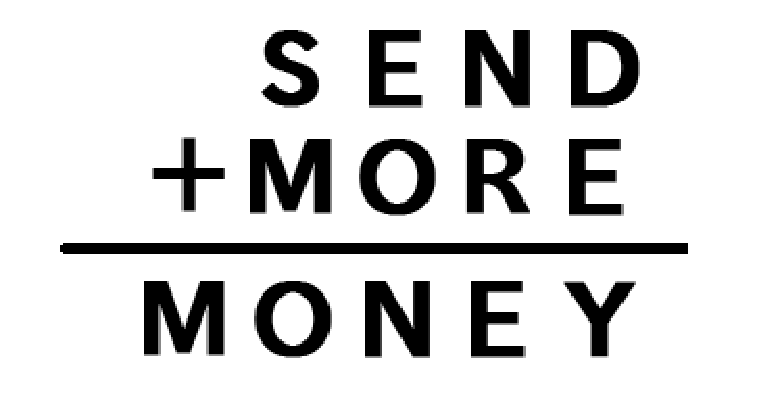
\epsfig{file=Figures/send-more-money.pdf, scale=0.4}}

\caption{A cryptarithmetic puzzle}
\label{fig:send-more-money.pdf}
\end{figure}


\noindent
A na\"ive approach to solve this problem would be to code it as a constraint satisfaction problem that has,
among others,  the
following constraint:
\\[0.2cm]
\hspace*{1.3cm}
$   (\mathtt{S} \cdot 10^3 + \mathtt{E} \cdot 10^2 + \mathtt{N} \cdot 10 + \mathtt{D}) 
  + (\mathtt{M} \cdot 10^3 + \mathtt{O} \cdot 10^2 + \mathtt{R} \cdot 10 + \mathtt{E})
  = \mathtt{M} \cdot 10^4 + \mathtt{O} \cdot 10^3 + \mathtt{N} \cdot 10^2 + \mathtt{E} \cdot 10 + \mathtt{Y}
$.
\\[0.2cm]
 The problem with this constraint is that it involves far too many variables.  As this constraint can only be
 checked when all the variables have values assigned to them, the backtracking search would essentially
 boil down to a mere brute force search.  In order to do better, we have to perform the addition in Figure
 \ref{fig:send-more-money.pdf} column by column, just as it is taught in elementary school.
 \myFig{send-more-money.stlx} shows how this can be implemented in \textsc{SetlX}.

\begin{figure}[!ht]
\centering
\begin{Verbatim}[ frame         = lines, 
                  framesep      = 0.3cm, 
                  firstnumber   = 1,
                  labelposition = bottomline,
                  numbers       = left,
                  numbersep     = -0.2cm,
                  xleftmargin   = 0.8cm,
                  xrightmargin  = 0.8cm,
                ]
    createCSP := procedure() {
        Variables   := { "S", "E", "N", "D", "M", "O", "R", "Y", "C1", "C2", "C3" };
        Values      := { 0 .. 9 };
        Constraints := allDifferent({ "S", "E", "N", "D", "M", "O", "R", "Y" });
        Constraints += { "(D + E) % 10 == Y", "(D + E) \\ 10 == C1",
                         "(N + R + C1) % 10 == E", "(N + R + C1) \\ 10 == C2",
                         "(E + O + C2) % 10 == N", "(E + O + C2) \\ 10 == C3",
                         "(S + M + C3) % 10 == O", "(S + M + C3) \\ 10 == M"
                       };
        Constraints += { "S != 0", "M != 0" };
        return [Variables, Values, Constraints];
    };
    allDifferent := procedure(Vars) {
        return { "$x$ != $y$" : x in Vars, y in Vars | x != y };
    };
\end{Verbatim}
\vspace*{-0.3cm}
\caption{Formulating ``$\mathtt{SEND} + \mathtt{MORE} = \mathtt{MONEY}$'' as a \textsc{Csp}.}
\label{fig:send-more-money.stlx}
\end{figure}

Notice that we have introduced three additional variables ``$\mathtt{C1}$'', ``$\mathtt{C2}$'', ``$\mathtt{C3}$''. 
These variables serve as the \href{https://en.wikipedia.org/wiki/Carry_(arithmetic)}{carry digits}.  For
example, ``$\mathtt{C1}$'' is the carry digit that we get when we do the addition of the last places of the two
numbers, i.e.~we have
\\[0.2cm]
\hspace*{1.3cm}
$\mathtt{D} + \mathtt{E} = \mathtt{C1} \cdot 10 + \mathtt{Y}$.
\\[0.2cm]
This equation still contains four variables.  We can reduce it to two equations that each involve only three
variables as follows:
\\[0.2cm]
\hspace*{1.3cm}
$(\mathtt{D} + \mathtt{E})\; \texttt{\symbol{37}}\; 10 = \mathtt{Y}$ \quad and \quad
$(\mathtt{D} + \mathtt{E}) \;\mathtt{\symbol{92}}\; 10 = \mathtt{C1}$.
\\[0.2cm]
Here, the symbol ``$\mathtt{\symbol{92}}$'' denotes 
\href{https://en.wikipedia.org/wiki/Division_(mathematics)#Of_integers}{integer division}, e.g.~we have $7 \mathtt{\symbol{92}} 3 = 2$.
If we try to solve the cryptarithmetic puzzle as coded in \myFig{send-more-money.stlx} using the
constraint solver developed in the previous section, we will be disappointed.  The reason is that most
constraints involve three variables and therefore the constraint propagation developed in the previous section
is of no help.  However, we can solve the problem in a few seconds if we add the following constraints for the
variables ``$\mathtt{C1}$'', ``$\mathtt{C2}$'', ``$\mathtt{C3}$'':
\\[0.2cm]
\hspace*{1.3cm}
\texttt{"C1 < 2", "C2 < 2", "C3 < 2"}.
\\[0.2cm]
Although these constraints are certainly true, the problem with this approach is that we would prefer if our
constraint solver would be able to figure out these constraints by itself.  After all, since $\mathtt{D}$ and
$\mathtt{E}$ are both less than $10$, there sum is obviously less than $20$ and hence the carry $\mathtt{C1}$
has to be less than $2$.  This line of reasoning is known as \emph{\color{blue}consistency maintenance}:
Assume that the formula $f$ is a constraint and the set of variables occurring in $f$ has the form
\\[0.2cm]
\hspace*{1.3cm}
$\mathtt{Var}(f) = \{ x \} + R$ \quad where $x \not\in R$,
\\[0.2cm]
i.e.~the variable $x$ occurs in the constraint $f$ and, furthermore, $R$ is the set of all variables occurring
in $f$ that are different from $x$.  Furthermore, assume that we have a dictionary $\mathtt{AllowableValues}$ such that
for every variable $y$, the dictionary entry $\mathtt{AllowableValues}[y]$ is the set of values that can be substituted
for the variable $y$.  Now  \emph{\color{blue}a value $v$ is consistent for $x$ with respect to the constraint $f$} 
iff the partial assignment $\{ \pair(x, v) \}$ can be extended to an assignment $A$ satisfying the constraint $f$,
i.e.~for every variable $y \in R$ we have to find a value $w \in \mathtt{AllowableValues}[y]$ such that the resulting
assignment $A$ satisfies the equations
\\[0.2cm]
\hspace*{1.3cm}
$\mathtt{evaluate}(f, A) = \mathtt{true}$.
\\[0.2cm]
Here, the function $\mathtt{evaluate}$ takes a formula $f$ and an assignment $A$ and evaluates $f$ using the
assignment $A$.  Now, \emph{\color{blue}consistency maintenance} works as follows.
\begin{enumerate}
\item The dictionary $\mathtt{AllowableValues}$ is initialized as follows:
      \\[0.2cm]
      \hspace*{1.3cm}
      $\mathtt{AllowableValues}[x] := \mathtt{Values}$ \quad for all $x \in \mathtt{Variables}$,
      \\[0.2cm]
      i.e.~initially every variable $x$ can take any value from the set of $\mathtt{Values}$.
\item Next, the set $\mathtt{UncheckedVariables}$ is initialized to the set of all $\mathtt{Variables}$:
      \\[0.2cm]
      \hspace*{1.3cm}
      $\mathtt{UncheckedVariables} := \mathtt{Variables}$.
\item As long as the set $\mathtt{UncheckedVariables}$ is not empty, we remove one variable $x$ from this set:
      \\[0.2cm]
      \hspace*{1.3cm}
      $x := \mathtt{from}(\mathtt{UncheckedVariables})$
\item We iterate over all constraints $f$ such that $x$ occurs in $f$.  
      \begin{enumerate}
      \item For every value $v \in \mathtt{AllowableValues}[x]$ we check whether $v$ is consistent with $f$.
      \item If $v$ is not consistent with $f$, then $v$ is removed from $\mathtt{AllowableValues}[x]$.
            Furthermore, if $R$ is the set of all variables occurring in $f$ that are different from $x$, 
            then this set $R$ is added to the set of $\mathtt{UncheckedVariables}$.
      \end{enumerate}
\item Once $\mathtt{UncheckedVariables}$ is empty, the algorithm terminates.  Otherwise, we jump back to step 3
      and remove the next variable from the set $\mathtt{UncheckedVariables}$.
\end{enumerate}
The algorithm terminates as every iteration removes either a variable from the set
$\mathtt{UncheckedVariables}$ or it removes a value from one of the sets $\mathtt{AllowableValues}[y]$ for some
variable $y$.  Now the set $\mathtt{UncheckedVariables}$ can grow during the algorithm, but the sets 
$\mathtt{AllowableValues}[y]$ can never grow.  However, every time the set $\mathtt{UncheckedVariables}$ grows,
the set $\mathtt{AllowableValues}[x]$ shrinks.
As the sets $\mathtt{AllowableValues}[y]$ are finite for all variables $y$, the set
$\mathtt{UncheckedVariables}$ can only grow a finite number of times. 
Once the set $\mathtt{UncheckedVariables}$ does not grow any more, every iteration of the algorithm removes one
variable from this set and hence the algorithm terminates eventually.

\begin{figure}[!ht]
\centering
\begin{Verbatim}[ frame         = lines, 
                  framesep      = 0.3cm, 
                  firstnumber   = 1,
                  labelposition = bottomline,
                  numbers       = left,
                  numbersep     = -0.2cm,
                  xleftmargin   = 0.0cm,
                  xrightmargin  = 0.0cm,
                ]
    enforceConsistency := procedure(rw ValuesPerVar, Var2Formulas, Annotated, Connected) {
        UncheckedVars := domain(Var2Formulas);
        while (UncheckedVars != {}) {
            variable    := from(UncheckedVars);
            Constraints := Var2Formulas[variable];
            Values      := ValuesPerVar[variable];
            RemovedVals := {};
            for (f in Constraints) {
                OtherVars := Annotated[f] - { variable };
                for (value in Values) {
                    if(!existsValue(variable, value, f, OtherVars, ValuesPerVar)) {
                        RemovedVals   += { value };
                        UncheckedVars += Connected[variable];
                    }
                }
            }
            Remaining := Values - RemovedVals;
            if (Remaining == {}) { backtrack; }
            ValuesPerVar[variable] := Remaining;
        }
    };
\end{Verbatim}
\vspace*{-0.3cm}
\caption{Consistency maintenance in \textsc{SetlX}.}
\label{fig:csp-consistency.stlx:enforceConsistency}
\end{figure}

\noindent
\myFig{csp-consistency.stlx:enforceConsistency} shows how consistency maintenance can be implemented in \textsc{SetlX}.
The procedure $\mathtt{enforceConsistency}$ takes four arguments.
\begin{enumerate}[(a)]
\item $\mathtt{ValuesPerVar}$ is a dictionary associating the set of possible values with each variable.
\item $\mathtt{Var2Formulas}$ is a dictionary.  For every variable $v$, $\mathtt{Var2Formulas}[v]$ is
      the set of those constraints $f$ such that $v$ occurs in $f$.
\item $\mathtt{Annotated}$ is the set of annnotated constraints, i.e. this set contains
      pairs of the form $\pair(f, V)$ where $f$ is a constraint and $V$ is the set of all variables occurring
      in $f$.  This last argument is needed only for efficiency: In order to avoid computing the set $V$ of
      variables occurring in a constraint $f$ every time the constraint $f$ is encountered, we compute these
      sets at the beginning of our computation and store them in the dictionary $\mathtt{Annnotated}$.
\item $\mathtt{Connected}$ is a dictionary that takes a variable $x$ and returns the set $V$ of all variables
      that are related to $x$ via a common constraint $f$, i.e.~we have $y \in \mathtt{Connected}[x]$
      if there exists a constraint $f$ such that both $x$ and $y$ occur in $f$ and, furthermore, $x \not= y$.
\end{enumerate}
The procedure $\mathtt{enforceConsistency}$ modifies the dictionary $\mathtt{ValuesPerVar}$ so that once the
procedure has terminated, for every variable $x$ the set
$\mathtt{ValuesPerVar}[x]$ is consistent with the constraints for $x$.  The implementation works as follows:
\begin{enumerate}
\item Initially, all variables need to be checked for consistency.  Therefore, $\mathtt{UncheckedVars}$
      is defined to be the set of all variables that occur in any of the constraints.
\item The \texttt{while}-loop iterates as long as there are still variables $x$ left in $\mathtt{UncheckedVars}$
      such that the consistency of $\mathtt{ValuesPerVar}[x]$ has not been established.
\item Next, a $\mathtt{variable}$ is selected and removed from $\mathtt{UncheckedVars}$. 
\item $\mathtt{Constraints}$ is the set of all constraints $f$ such that this $\mathtt{variable}$ occurs in $f$.
\item $\mathtt{Values}$ is the set of those values that can be assigned to $\mathtt{variable}$.
\item $\mathtt{RemovedVals}$ is the subset of those values that are found to be inconsistent with some constraint.
\item We iterate over all constraints $\mathtt{f} \in \mathtt{Constraints}$.
\item $\mathtt{OtherVars}$ is the set of variables occurring in $\mathtt{f}$ that are different from 
      the chosen $\mathtt{variable}$.
\item We iterate over all $\mathtt{value} \in \mathtt{Values}$ that can be substituted for $\mathtt{variable}$
      and check whether $\mathtt{value}$ is consistent with $\mathtt{f}$.   To this end, we need to find values
      that can be assigned to the variables in the set $\mathtt{OtherVars}$ such that $\mathtt{f}$ evaluates as
      $\mathtt{true}$.  This is checked using the function $\mathtt{existsValue}$.
\item If we do not find such values, then $\mathtt{value}$ is inconsistent for
      $\mathtt{variable}$ w.r.t.~$\mathtt{f}$ and needs to be removed from the set 
      $\mathtt{ValuesPerVar}[\mathtt{variable}]$.  Furthermore, all variables that are connected to
      $\mathtt{variables}$ have to be added to the set $\mathtt{UncheckedVars}$.  The reason is that once a
      value is removed for $\mathtt{variable}$, the value assigned to another variable $y$ occurring in a
      constraint that mentions both $\mathtt{variable}$ and $y$ might now become inconsistent.
\item If there are no consistent values for $\mathtt{variable}$ left, we have to backtrack.
\end{enumerate}

\begin{figure}[!ht]
\centering
\begin{Verbatim}[ frame         = lines, 
                  framesep      = 0.3cm, 
                  firstnumber   = 1,
                  labelposition = bottomline,
                  numbers       = left,
                  numbersep     = -0.2cm,
                  xleftmargin   = 0.8cm,
                  xrightmargin  = 0.8cm,
                ]
    existsValue := procedure(var, val, f, Vars, ValuesPerVar) {
        AllVars := { var } + Vars;
        for (A in createAllAssignments(Vars, ValuesPerVar)) {
            if (eval_constraint(A + { [var, val] }, f, AllVars)) {
                return true;
            }
        }
        return false;    
    };
    createAllAssignments := procedure(Vars, ValuesPerVar) {
        if (Vars == {}) {
            return { {} };  // set containing empty assignment
        }
        var         := from(Vars);
        Values      := ValuesPerVar[var];
        Assignments := createAllAssignments(Vars, ValuesPerVar);
        return { { [var, val] } + A : val in Values, A in Assignments };
    };
\end{Verbatim}
\vspace*{-0.3cm}
\caption{The implementation of $\mathtt{existsValue}$.}
\label{fig:csp-consistency.stlx:existsValue}
\end{figure}

\noindent
\myFig{csp-consistency.stlx:existsValue} shows the implementation of the function $\mathtt{existsValue}$ that
is used in the implementation of $\mathtt{enforceConsistency}$.  This procedure is called with five arguments.
\begin{enumerate}[(a)]
\item $\mathtt{var}$ is variable.
\item $\mathtt{val}$ is a value that is to be assigned to $\mathtt{var}$.
\item $\mathtt{f}$ is a constraint such that $\mathtt{var}$ occurs in $\mathtt{f}$
\item $\mathtt{Vars}$ is the set of all those other variables occurring in $\mathtt{f}$, i.e.~the set of those
      variables that occur in $\mathtt{f}$ but that are different from $\mathtt{var}$. 
\item $\mathtt{ValuesPerVar}$  is a dictionary associating the set of possible values with each variable.
\end{enumerate}
The procedure checks whether the partial assignment $\{ \pair(\mathtt{var}, \mathtt{val}) \}$ can be
extended so that the constraint $\mathtt{f}$ is satisfied.  To this end it needs to create the set of all
possible assignments.  This set is generated using the function $\mathtt{createAllAssignments}$.  This function
gets a set of variables $\mathtt{Vars}$ and a dictionary that assigns to every variable $\mathtt{var}$ in
$\mathtt{Vars}$ the set of values that might be assigned to $\mathtt{var}$.
\begin{enumerate}
\item If the set of variables $\mathtt{Vars}$ is empty, the empty set can serve as a dictionary that 
      assigns a value to every variable in $\mathtt{Vars}$.
\item Otherwise, we remove a variable $\mathtt{var}$ from $\mathtt{Vars}$ and get the set of $\mathtt{Values}$
      that can be assigned to $\mathtt{var}$.  
\item Recursively, we create the set of all $\mathtt{Assignments}$ that associate values with the remaining 
      variables.
\item Finally, the set of all possible assignments is the set of all combinations of assigning a value 
      $\mathtt{val} \in \mathtt{Values}$ to $\mathtt{var}$ and assigning the remaining variables according to 
      an assignment $\mathtt{A} \in \mathtt{Assignments}$.
\end{enumerate}
On one hand, consistency checking creates a lot of overhead.\footnote{
  To be fair, the implementation shown in this section is far from optimal.  In particular, by remembering which
  combinations of variables and values work for a given formula, the overhead can be reduced greatly.  I have
  refrained from implementing this optimization because I did not want the code to get too complex.
}
Therefore, it might actually slow down the
solution of some constraint satisfaction problems that are easy to solve using just backtracking and
propagation.  On the other hand, many difficult constraint satisfaction problems can not be solved
without consistency checking.

\section{Local Search}
There is another approach to solve constraint satisfaction problems.  This approach is known as
\emph{\color{blue}local search}.  The basic idea is simple: Given as constraint satisfaction problem 
$\mathcal{C}$ of the form 
\\[0.2cm]
\hspace*{1.3cm}
$\mathcal{P} := \langle \mathtt{Variables}, \mathtt{Values}, \mathtt{Constraints} \rangle$,
\\[0.2cm] 
local search works as follows:
\begin{enumerate}
\item Initialize the values of the variables in $\mathtt{Variables}$ randomly.  
\item If all $\mathtt{Constraints}$ are satisfied, return the solution.
\item For every  $x \in \mathtt{Variables}$, count the number of \underline{unsatisfied} constraints that involve the
      variable $x$. 
\item Set $\mathtt{maxNum}$ to be the maximum of these numbers, i.e.~$\mathtt{maxNum}$ is maximal number of
      unsatisfied constraints for any variable.
\item Compute the set $\mathtt{maxVars}$ of those variables that have $\mathtt{maxNum}$ unsatisfied constraints.
\item Randomly choose a variable $x$ from the set $\mathtt{maxVars}$.
\item Find a value $d \in \mathtt{Values}$ such that by assigning $d$ to the variable $x$, the number of
      unsatisfied constraints for the variable $x$ is minimized.  

      If there is more than one value $d$ with this property, choose the value $d$ randomly from those values
      that minimize the number of unsatisfied constraints.
\item Goto step 2 and repeat until either a solution is found or the sun rises in the west.
\end{enumerate}

\begin{figure}[!ht]
\centering
\begin{Verbatim}[ frame         = lines, 
                  framesep      = 0.3cm, 
                  firstnumber   = 1,
                  labelposition = bottomline,
                  numbers       = left,
                  numbersep     = -0.2cm,
                  xleftmargin   = 0.8cm,
                  xrightmargin  = 0.8cm,
                ]
    solve := procedure(n) {
        Queens := [];
        for (row in [1 .. n]) {
            Queens[row] := rnd({1 .. n});
        }
        iteration := 0;
        while (true) {
            Conflicts   := { [numConflicts(Queens, row), row] : row in [1 ..n] };
            [maxNum, _] := last(Conflicts);
            if (maxNum == 0) {
                return Queens;
            }
            if (iteration % 10 != 0) { // avoid infinite loops
                row := rnd({ row : [num, row] in Conflicts | num == maxNum });
            } else {
                row := rnd({ 1 .. n });
            }
            Conflicts := {};
            for (col in [1 .. n]) {
                Board      := Queens;
                Board[row] := col;
                Conflicts  += { [numConflicts(Board, row), col] };
            }
            [minNum, _] := first(Conflicts);
            Queens[row] := rnd({ col : [num, col] in Conflicts | num == minNum });
            iteration   += 1;
        }
    };
\end{Verbatim}
\vspace*{-0.3cm}
\caption{Solving the $n$ queens problem using local search.}
\label{fig:constraints.stlx}
\end{figure}

\noindent
\myFig{constraints.stlx} shows an implementation of these ideas in \textsc{SetlX}.  Instead of solving an
arbitrary constraint satisfaction problem, the program solves the $n$ queens problem.  We proceed to discuss
this program line by line.
\begin{enumerate}
\item The procedure $\mathtt{solve}$ takes one parameter $\mathtt{n}$, which is the size of the chess board.  If
      the computation is successful, $\mathtt{solve(n)}$ returns a list of length $\mathtt{n}$.  Lets call this
      list $\mathtt{Queens}$. For every row $\mathtt{r} \in \{1, \cdots, \mathtt{n}\}$, the value $\mathtt{Queens[r]}$ specifies that the queen 
      that resides in row $\mathtt{r}$ is positioned in column $\mathtt{Queens[r]}$.
\item The \texttt{for} loop initializes the positions of the queens to random values from the set
      $\{1, \cdots, \mathtt{n}\}$.  Effectively, for every row on the chess board, this puts a queen in a
      random column.
\item The variable $\mathtt{iteration}$ counts the number of times that we need to reassign a queen in a given row.
\item All the remaining statements are surrounded by a \texttt{while} loop that is only terminated once a
      solution has been found.
\item The variable $\mathtt{Conflicts}$ is a set of pairs of the form $[c, r]$, where $c$ is the number of
      times the queen in row $r$ is attacked by other queens.  Hence, $c$ is the same as the number of
      unsatisfied conflicts for the variable specifying the column of the queen in row $r$.
\item $\mathtt{maxNum}$ is the maximum of the number of conflicts for any row.
\item If this number is $0$, then all constraints are satisfied and the list $\mathtt{Queens}$ is a solution to the
      $\mathtt{n}$ queens problem.
\item Otherwise, we compute those rows that exhibit the maximal number of conflicts.  From these rows
      we select one $\mathtt{row}$ arbitrarily.
\item The reason for enclosing the assignment to $\mathtt{row}$ in an \texttt{if} statement is explained later. 
      On a first reading of  this program,  this \texttt{if} statement should be ignored.
\item Now that we have identified the $\mathtt{row}$ where the number of conflicts is biggest, we need to
      reassign $\mathtt{Queens[row]}$.  Of course, when reassigning this variable, we would like to have fewer
      conflicts after the reassignment.  Hence, we test all columns to find the best column that can be
      assigned for the queen in the given $\mathtt{row}$.  This is done in a \texttt{for} loop that runs over
      all possible columns.  The set $\mathtt{Conflicts}$ that is maintained in this loop is a set of pairs
      of the form $[k, c]$ where $k$ is the number of times the queen in $\mathtt{row}$ would be attacked if it
      would be placed in column $c$.
\item We compute the minimum number of conflicts that is possible for the queen in $\mathtt{row}$ and assign it
      to $\mathtt{minNum}$.
\item From those columns that minimize the number of violated constraints, we choose a column randomly
      and assign it for the specified $\mathtt{row}$.
\end{enumerate}
There is a technical issue, that must be addressed:  It is possible there is just one row that exhibits the
maximum number of conflicts.  It is further possible that, given the placements of the other queens, there is
just one optimal column for this row.  In this case, the procedure $\mathtt{solve}$ would loop forever.  To
avoid this case, every 10 iterations we pick a random row to change.

\begin{figure}[!ht]
\centering
\begin{Verbatim}[ frame         = lines, 
                  framesep      = 0.3cm, 
                  firstnumber   = 1,
                  labelposition = bottomline,
                  numbers       = left,
                  numbersep     = -0.2cm,
                  xleftmargin   = 0.8cm,
                  xrightmargin  = 0.8cm,
                ]
    numConflicts := procedure(Queens, row) {
        n      := #Queens;
        result := 0;
        for (r in {1 .. n} | r != row) {
            if ( Queens[r] == Queens[row]           ||
                 r - Queens[r] == row - Queens[row] ||
                 r + Queens[r] == row + Queens[row]
               )
            { result += 1; }
        }
        return result;
    };
\end{Verbatim}
\vspace*{-0.3cm}
\caption{The procedure $\mathtt{numConficts}$.}
\label{fig:numConficts.stlx}
\end{figure}

The procedure $\mathtt{numConficts}$ shown in \myFig{numConficts.stlx} implements the function
$\mathtt{numConficts}$.  Given a board $\mathtt{Queens}$ that specifies the positions of the queens on the
board and a $\mathtt{row}$, this function computes the number of ways that the queen in $\mathtt{row}$ is
attacked by other queens.  If all queens are positioned in different rows, then there are only three ways left
that a queen can be attacked by another queen.
\begin{enumerate}
\item The queen in row $\mathtt{r}$ could be positioned in the same column as the queen in $\mathtt{row}$.
\item The queen in row $\mathtt{r}$ could be positioned in the same falling or rising diagonal as the queen in
      $\mathtt{row}$.  These diagonals are specified by the linear equations given in line 6 and 7 of Figure
      \ref{fig:numConficts.stlx}.
\end{enumerate}
Using the program discussed in this section, the n queens problem can be solved for a $\mathtt{n} = 1000$ in
30 minutes.  As the memory requirements for local search are small, even much higher problem sizes can be
tackled if sufficient time is available.  Hence, it seems that local search is much better than the algorithms
discussed previously.  However, we have to note that local search is \emph{\color{blue}incomplete}:  If a
constraint satisfaction problem $\mathcal{P}$ has no solution, then local search loops forever.  Therefore, in
practise a dual approach is used to solve a constraint satisfaction problem.  The constraint solver starts two
threads: The first search does local search, the second thread tries to solve the problem via some refinement
of backtracking.  the first thread that terminates wins.  The resulting algorithm is complete and, for a
solvable problem, will have similar performance as local search.  If the problem is unsolvable, this will
\emph{\color{blue}eventually} be discovered by backtracking.  Note, however, that the constraint satisfaction
problem is NP-complete.  Hence, it is unlikely that there is an efficient algorithm that works always.
However, many practically occurring constraint satisfaction problems can be solved today in a reasonably short
time. 

%%% Local Variables:
%%% mode: latex
%%% TeX-master: "artificial-intelligence"
%%% End:
